\documentclass[11pt, notitlepage,preprint]{report}   % [put font size 10-11-12]

%%%%%%%%%%%%%%%%%%%%%%%%%%%%%%%%%%%%%%%%%%%%%%%%%%%%%%%%%
%%%%%%% put packages required all over the thesis %%%%%%%
%%%%%%%%%%%%%%%%%%%%%%%%%%%%%%%%%%%%%%%%%%%%%%%%%%%%%%%%%
\usepackage[utf8]{inputenc}

%%%% EDITING OF PAGE FRAME %%%%
%\usepackage{showframe}          %This line can be used to clearly show the new margins

%\usepackage{a4wide}            % Unblock this package if you prefer the text to be wider on the page (more MS-like)
\usepackage{geometry}
\newgeometry{vmargin={35mm}, hmargin={30mm,29mm}}   % set the margins (in a book format, it is useful not to shrink too much the margins)
\usepackage{changepage}         % useful to locally change margin (used in specimen)
\usepackage{fancyhdr}           % useful for headers editing

%%%% LINE, PARAGRAPH, IDENTATION %%%%
\setlength{\parindent}{2em}             % indentation for § start
\setlength{\parskip}{0.5em}             % paragraph spacing
\renewcommand{\baselinestretch}{1}      % line spacing

%%%% LANGUAGE %%%%
\usepackage[english]{babel}
\usepackage{dirtytalk}          % useful for quotation marks put in a causual way
\usepackage{textgreek}      
\usepackage{lipsum}

%%%% OTHER SECONDARY EDITING 
\usepackage{copyrightbox}       % useful for the page 3 of the specimen
\usepackage{textcomp}           % useful for the gensymb package
\usepackage{gensymb}            % required to put the "degree" symbol "°"C 
\usepackage{lineno}             % useful in case the line number is required (for some reason)      \linenumbers
\usepackage{epigraph}           % useful for quotation before chapter, etc.
\renewcommand{\textflush}{flushepinormal} % justify epigraph
\usepackage{pdflscape}          % useful to put landscape (e.g. for large tables)
\usepackage{lscape}             % useful to put landscape (e.g. for large tables)
\usepackage{wrapfig}            % useful some text wrapping around figures
\usepackage{pdfpages}           % useful to include the imprimatur
\usepackage{rotating}           % useful to rotate some content
%\usepackage{fontspec}          % useful for some other font, e.g. Arial font, but need another LaTeX

%%%% MORE CONTENT %%%%
\usepackage{longtable}          % useful for long table, crossing pages
\usepackage[flushleft]{threeparttable}
\usepackage{multirow}           % useful for table editing
\usepackage{subcaption}         % useful to edit table, figure, etc. captions
\usepackage{booktabs,caption}   % useful for caption alignment
\usepackage{graphicx}           % useful for inclusion of image and other content
\usepackage{float}              % useful for positioning of content (e.g. of tables)
\usepackage{etoolbox}           % useful if you use macro
\usepackage{epstopdf}           % useful in case you need EPS to be encapsulated into PDF

%%%% MATH SYMBOLS %%%%
\usepackage{amssymb}            % useful mathematical symbols
\usepackage{amsmath}            % useful mathematical symbols
\usepackage{mathrsfs}           % useful for mathematical fonts
\newcommand{\R}{\mathbb{R}}     % useful to give elegant letters
\usepackage{chngcntr}           % useful in case a different counting of propositions, etc. is required

%%%% Hyperreferencing %%%% 
\usepackage{hyperref}           % useful for referencing outside the present document
\hypersetup{
    colorlinks=true,
    linkcolor=black,
    filecolor=magenta,      
    urlcolor=cyan,
    citecolor=black     %blue,
}

%%%% APPENDICES %%%%
%\usepackage{appendix}
\usepackage[toc,page]{appendix}     % useful to have table of contents for appendix 
\AtBeginEnvironment{subappendices}{ % needed to have correct appendices in each article 
\chapter*{Appendix}
\addcontentsline{toc}{chapter}{Appendices}
\counterwithin{figure}{section}
\counterwithin{table}{section}
}

%%%% BIBLIOGRAPHY %%%%
\usepackage[sectionbib]{natbib}     % required to have one biblio per chapter
\usepackage{chapterbib}             % required to have one biblio per chapter


%%%%%%%%%%%%%%%%%%%%%%%%%%%%%%%%%%%%%%%%%%%%%%%%%%%%%%%%%%
%%%%%%%%%%%%%%%%%%%%%%%%%%%%%%%%%%%%%%%%%%%%%%%%%%%%%%%%%%
%%%%% Define newcommand for your personnal information on the first pages %%%%%
\newcommand{\MyTitle}{\# Essays in ... (or whatever title)} % 
\newcommand{\ThesisNumber}{Thesis Number}                   % It will be given by the secretariat
\newcommand{\ThesisMajor}{International Economics}          % Development Economics
\newcommand{\YearRegistration}{\the\year}                     % In case you submit around the Winter Break, just make sure that this is correct   
\newcommand{\City}{Geneva}  

\newcommand{\MyName}{Name}                                  % You must use the name the institute registered you in
\newcommand{\MySurname}{ \MakeUppercase{Surname}}           % note that the space before the "\MakeUppercase" command matters
%%%%%%%%%%%%%%%%%%%%%%%%%%%%%%%%%%%%%%%%%%%%%%%%%%%%%%%%%%
%%%%%%%%%%%%%%%%%%%%%%%%%%%%%%%%%%%%%%%%%%%%%%%%%%%%%%%%%%



%%%%%%%%%%%%%%%%%%%%%%%%%%%%%%%%%%%%%%%
%%%%%%%%%%%%%%%%%%%%%%%%%%%%%%%%%%%%%%%
%%%%%%% IHEID-BASED FIRST PAGES %%%%%%%
%%%%%%%%%%%%%%%%%%%%%%%%%%%%%%%%%%%%%%%
%%%%%%%%%%%%%%%%%%%%%%%%%%%%%%%%%%%%%%%
% Same frame for 1st and 3rd page
\makeatletter
\renewcommand\maketitle
    {\vspace*{3cm} 
    \begin{center}
        \Large\sffamily\textbf{\MyTitle}                \\[5\baselineskip]
        \large\sffamily\textbf{THESIS}                  \\[0\baselineskip] 
        submitted at the Graduate Institute             \\[0\baselineskip] 
        in fulfillment of the requirements of the       \\[0\baselineskip] 
        PhD degree in \ThesisMajor                      \\[2\baselineskip]
        \large\sffamily{by                              \\[2\baselineskip] 
        \textbf{	\MyName 	\MySurname}
        }
        \bigskip                                        \\[0\baselineskip]
    \end{center}
    }

%%%%%%%%%%%%%%%%%%%%%%%%%%%%%
%%%%%%%%%%%%%%%%%%%%%%%%%%%%%
\begin{document}
%%%%%%%%%%%%%%%%%%%%%%%%%%%%%
%%%%%%%%%%%%%%%%%%%%%%%%%%%%%
%%% TITLEPAGES %%%
%%%%%%%%%%%%%%%%%
%%% TITLEPAGE 1 %%%
\begin{titlepage}
    \begin{tikzpicture}[remember picture,overlay]           % put the logo on the top-left corner
        \node[anchor=north west,yshift=-25pt,xshift=25pt]%
        at (current page.north west)
        {\includegraphics[width=0.5\textwidth]{logo.png}};
    \end{tikzpicture}
    \maketitle
    \vspace{1cm}
    \centering\sffamily{Thesis N$^{\circ}$ \ThesisNumber}     \\[0.5\baselineskip] 
    \vspace{1cm}
    \centering\sffamily\textbf{\City}                         \\[0.5\baselineskip]
    \vspace{1cm}
    \centering\sffamily\textbf{\YearRegistration}
\end{titlepage}
%%% TITLEPAGE 2 %%% (empty page)
\newpage\null\thispagestyle{empty}\newpage
%%% TITLEPAGE 3 %%%
\begin{titlepage}
    \vspace*{5cm}
    \centering\Large\sffamily\textbf{\MyTitle}
    \vspace*{10cm} \\
    \large\raisebox{0.1em}{\textcopyright} \sffamily\textbf{\YearRegistration} \hspace{1em} \sffamily \textbf{\MyName \MySurname}
\end{titlepage}
%%% TITLEPAGE 4 %%%
\begin{titlepage}
    \begin{adjustwidth}{-20pt}{-20pt}
        \begin{center}
            \sffamily{
            INSTITUT DE HAUTES ETUDES INTERNATIONALES ET DU DEVELOPPEMENT   \\[0.5\baselineskip]
            GRADUATE INSTITUTE OF INTERNATIONAL AND DEVELOPMENT STUDIES      }   
        \end{center}
    \end{adjustwidth}           
    \vspace{1cm}
    \maketitle
    \vspace{1cm}
    \centering\sffamily{Thesis N$^{\circ}$\ThesisNumber}  \\[0.5\baselineskip] 
    \vspace{1cm}
    \centering\sffamily\textbf{\City}                     \\[0.5\baselineskip]
    \vspace{1cm}
    \centering\sffamily\textbf{\YearRegistration}
\end{titlepage}
%%% TITLEPAGE 5 %%%

\includepdf[pages={1}]{IMPRIMATUR.pdf}
%%% TITLEPAGE 6 %%%
\begin{titlepage}   
\pagenumbering{roman}       % use roman numbering for the first pages (outside the specimen, not counted)
\setcounter{page}{0}        % start the roman page count after the 6 pages specimen 
%%%%%%%%%%%%%%%%%%%%%%%%%%%%%
%%%%%%%%%%%%%%%%%%%%%%%%%%%%%

\vspace*{-3.5cm}

\begin{center}
\sffamily\large\textbf{RESUME / ABSTRACT}
\end{center}

\noindent   Titre de la thèse / Title of thesis: FSDJFGHDJV

\noindent   \sffamily\textit{Résumé en français :} \sffamily{
\begin{small}
\lipsum[2-2]
\end{small}
}

\noindent   \sffamily\textit{English Summary:}  \sffamily{
\begin{small}
\lipsum[4-4]
\end{small}
}
%%%%%%%%%%%%%%%%%%%%%%%%%%%%%
%%%%%%%%%%%%%%%%%%%%%%%%%%%%%   
%%%%%%%%%%%%%%%%%
% END TITLE PAGES
%%%%%%%%%%%%%%%%%
%%%%%%%%%%%%%%%%%
%%%%%%%%%%%%%%%%%
% MAIN CONTENT   %\maketitle
%%%%%%%%%%%%%%%%%
%%%%%%%%%%%%%%%%%
\newpage
\vspace*{6cm}
\setlength\epigraphwidth{10cm}
\setlength\epigraphrule{0pt}
          \begin{flushright}
\textit{Quote, if willing to!} \\[0.5\baselineskip]
\textbf{\textit{Author}}
          \end{flushright}  
%%
\newpage
\vspace*{6cm}
\setlength\epigraphwidth{10cm}
\setlength\epigraphrule{0pt}
          \begin{flushright}
\textit{I dedicate this thesis to the golden shrimp.} \\[0.5\baselineskip]
          \end{flushright}
%%%%%%%%%%%%%%%%%%%%%%%%%%%%%
\chapter*{Acknowledgments}


\lipsum[5-5]
%%%%%%%%%%%%%%%%%%%%%%%%%%%%%
\tableofcontents
%\listoffigures         % list of figures           
%\listoftables          % list of tables
%%%%%%%%%%%%%%%%%%%%%%%%%%%%%
\end{titlepage}
\pagenumbering{arabic}      % put back the arabic numbering
\setcounter{page}{1}        % start the main page count after the table(s) of contents, quotes, etc.
%%%%%%%%%%%%%%%%%%%%%%%%%%%%%
% The key aspects to preserve are the \chapter, and the \bibliography commands. For the rest, there should be full flexibility
\chapter*{Preamble}



\lipsum[7-7], as in \citet{borjas1991immigration}, ... 


%%%%%%%%
\newpage
\bibliographystyle{chicago}
\bibliography{Bibliographies/Preamble.bib}
%%%%%%%%%%%%%%%%%%%%%%%%%%%%%
% The key aspects to preserve are the \chapter, the \bibliography, and the \subappendices commands. For the rest, there should be full flexibility
\chapter{Title paper 1}

%% Text of abstract
\begin{abstract}
\noindent   \lipsum[9-9]
\end{abstract}

\noindent   \textit{Keywords:}      \newline
            \textit{JEL Codes:}



\pagebreak
\setlength\epigraphwidth{10cm}
\setlength\epigraphrule{0pt}
\epigraph{      \flushright{\textit{Quote for Paper 1}} }   

% main text
\section{Introduction}

% For example, I implement this strategy... 

\lipsum[11-11] Table (\ref{paper1_summary_stat}) shows...

\begin{table}[ht]
    \centering
{
\def\sym#1{\ifmmode^{#1}\else\(^{#1}\)\fi}
\begin{tabular}{l*{1}{ccccc}}
\hline\hline
       %             &Summary Statistics&            &            &            &            \\
                    &Observations&        Mean&          SD&         Min&         Max\\
\hline
Price               &          74&    6165.257&  (2949.496)&    3291.000&   15906.000\\
Mileage             &          74&      21.297&     (5.786)&      12.000&      41.000\\
Repair              &          69&       3.406&     (0.990)&       1.000&       5.000\\
Headroom            &          74&       2.993&     (0.846)&       1.500&       5.000\\
Trunk               &          74&      13.757&     (4.277)&       5.000&      23.000\\
Weight              &          74&    3019.459&   (777.194)&    1760.000&    4840.000\\
Length              &          74&     187.932&    (22.266)&     142.000&     233.000\\
\hline\hline
\end{tabular}
}
\caption{Summary Statistics}
\label{paper1_summary_stat}
\end{table}  




\section{The analysis}

\lipsum[8-8] As in table (\ref{paper1_table_frequency}). The first mention of an acronym refers to what it means: \gls{usa} (as described in \citet{krugman2010theory}). And there is \cite{woessmann2016importance}...

\begin{center}
    \vspace{0.3cm}
    \textit{[Table \ref{paper1_table_frequency}]}
    \vspace{0.3cm}
\end{center}

\begin{figure}[hbt!]
    \centering
    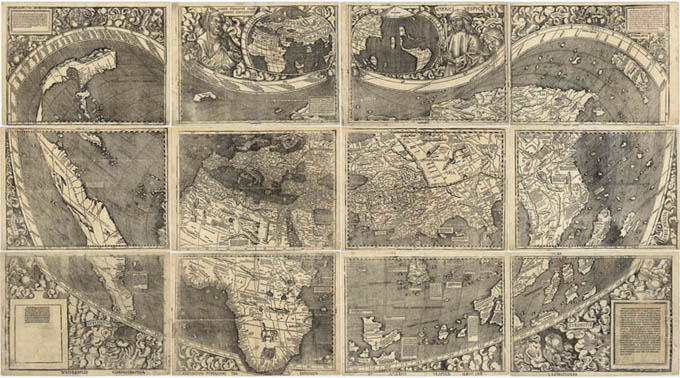
\includegraphics[width=0.9\textwidth]{graph_and_picture/Waldseemuller_map.jpg}
    \caption{A map}
    \label{chapter1_map_waldseemuller}
\end{figure}



% Bibliography Paper 1
\pagebreak
\bibliographystyle{\stylechoice}
\bibliography{Bibliographies/Paper1.bib}


% If you put main tables/maps/graph, etc. outside the main text but not in Appendix:
\pagebreak
\section*{Tables (if put in the end of the paper)}

\begin{table}[h!]
    \centering
    \begin{tabular}{cccc}
\hline \hline
\multirow{2}{*}{Frequency} &   & \multicolumn{2}{l}{Region}       \\
                           &   & A           & B                  \\
\hline                           
\multirow{2}{*}{Period}    & 1 & 78521          & 3982            \\
                           & 2 & 54246          & 3521            \\
\hline \hline
    \end{tabular}
    \caption{Frequency Table}
    \label{paper1_table_frequency}
\end{table}  



% Appendices Paper 1
\pagebreak
\begin{subappendices}

\section{The colors on the maps}
\lipsum[10-10]

\section{{The origin of the map}}
\lipsum[11-11]


\end{subappendices}
%%%%%%%%%%%%%%%%%%%%%%%%%%%%%
% The key aspects to preserve are the \chapter, the \bibliography, and the \subappendices commands. For the rest, there should be full flexibility
\chapter{Paper 2}

\begin{abstract}
\end{abstract}

\noindent   \textit{Keywords:}      \newline
            \textit{JEL Codes:}



\pagebreak
% main text
\section{Introduction}\label{Paper2_intoduction}

The second reference of an acronym does not express what it means: \Gls{usa}.


% Bibliography Paper 2
\pagebreak
\bibliographystyle{\stylechoice}
\bibliography{Bibliographies/Paper2.bib}


% Appendices Paper 2
\pagebreak
\begin{subappendices}

\section{Appendix 1}\label{app_1}
 

\end{subappendices}
%%%%%%%%%%%%%%%%%%%%%%%%%%%%%
% The key aspects to preserve are the \chapter, the \bibliography, and the \subappendices commands. For the rest, there should be full flexibility
\chapter{Paper 3}

\begin{abstract}
\end{abstract}

\noindent   \textit{Keywords:}      \newline
            \textit{JEL Codes:}



\pagebreak
% main text
\section{Introduction}



\pagebreak
\bibliographystyle{chicago}
\bibliography{Bibliographies/Paper3.bib}



\pagebreak
\begin{subappendices}

\section{Appendix 1}

\end{subappendices}
%%%%%%%%%%%%%%%%%%%%%%%%%%%%%
%%%%%%%%%%%%%%%%%%%%%%%%%%%%%
\end{document}
%%%%%%%%%%%%%%%%%%%%%%%%%%%%%
%%%%%%%%%%%%%%%%%%%%%%%%%%%%%